\documentclass{article}
\usepackage[utf8]{inputenc}
\usepackage{graphicx}

\title{LabMuoni}
\author{giulia lavizzari}
\date{November 2021}

\begin{document}

\maketitle

\section{12/11/21}
Primo approcio alla strumentazione. Sembrava ancora che le cose funzionassero :)

\section{17/11/21}
Caratterizzazione dei moduli
\\\\\textbf{Discriminator threshold settings:}
\begin{itemize}
    \item range threshold
    \item corrispondenza tra valore della soglia e altezza dell'impulso
\end{itemize}\
\textbf{Timer counter settings:}
\begin{itemize}
    \item lo stesso numero di conteggi viene osservato con tutti i canali (impulsatore $\rightarrow$ discriminatore con soglia bassa $\rightarrow$ counter)
\end{itemize}


\section{19/11/21}
\textbf{Caratterizzazione dei moduli con impulsatore (onde quadre) e caratterizzazione risposta scintillatore con scelta della soglia}\\\\
Carattatterizzazione nuovo discriminatore: range soglia per ogni canale, risposta corretta del modulo all'onda quadra.\\\\
Scelta della soglia: discriminatore + scintillatore zero. Plot rate vs thr, si cerca il plateau. HV = 900V, t=100s
\begin{figure}
    \centering
    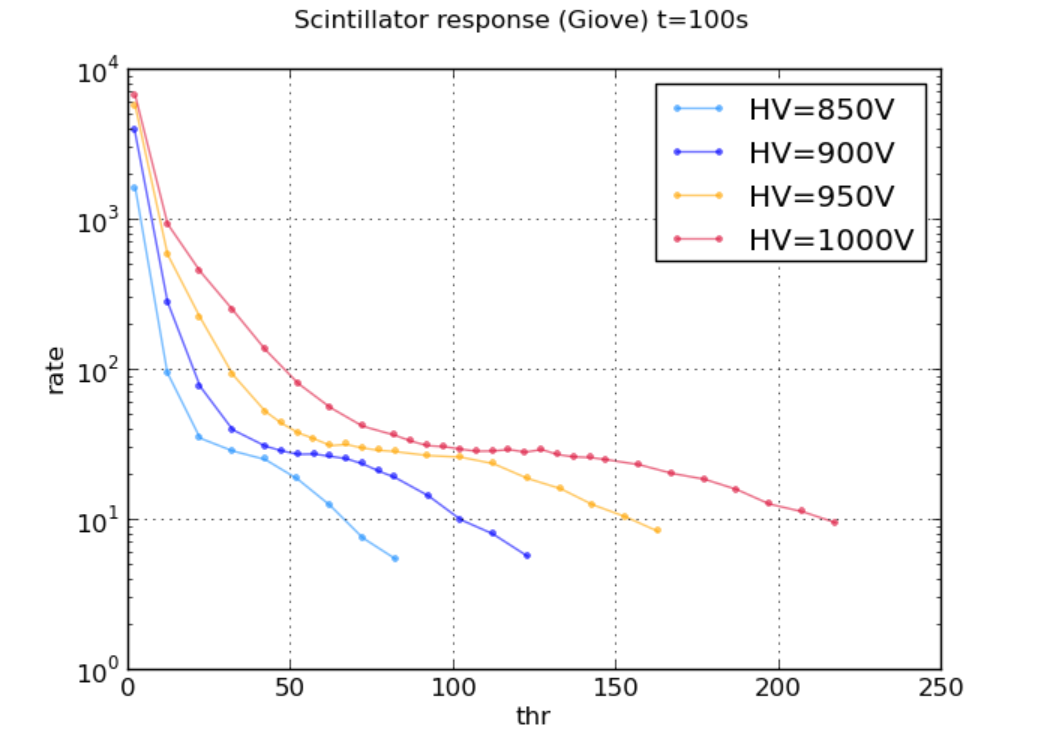
\includegraphics[width=0.9\textwidth]{dati1.PNG}
\end{figure}



\section{24/11/21}
\textbf{scelti i nomiii}
Giove (G1)
Giunone (G2)
Minerva (M)\\\\
\textbf{caratterizzazione risposta scintillatore al variare della soglia}\\
Caratterizzazione della risposta di ciascuno dei tre scintillatori.\\\\
Tip per il futuro: valutare la tensione di bias di Minerva in base alle efficienze: siccome per Minerva non si vede bene il plateau, è difficile scegliere la soglia e bias. Ci si mette in una situa in cui G1 - M - G2 e con soglie di G1 e G2 tali da essere nel plateau (così per loro siamo sicuri di beccare i muoni). Se vedo una coinc per G1 e G2 ma non per M vuol dire che sto tagliando i muoni, quindi regolare thr e bias di M.\\\\
\textbf{giulia ha scoperto i colori ;)}
Siamo felici :D \\\\


\section{26/11/21}
Stiamo andanso avanti con la stessa cosa. Oggi siamo meno felici. Abbiamo però scoperto che il primo punto dei grafici (soglia bassissima, 2mV) ha un rate sovrastimato perchè al passaggio di un singolo impulso si aprono più finestre nel discriminatore. Questo già da 12mV non succede più (per Minerva abbiamo ampliato la finestra temporale affinchè non succedesse)\\\\
\textbf{Finestra temporale discr:} 65ns per G1,G2 - 80s per M

\section{01/12/21}
Caro diario,\\
Niente di nuovo sul fronte occidentale. Andiamo avanti con le misure. Speriamo di vedere qualche plateau per Minerva. Nessun plateau è stato trovato per Minerva. Ma vabbé.\\\\
Recuperiamo i moduli per fare le misure con le efficienze (non caratterizziamo i moduli, ci fidiamo perchè dobbiamo fare le misure prima di Natale)


\end{document}